\chapter{Hardware di destinazione}
    
Come precedentemente scritto nell'introduzione, la scelta di utilizzare la scheda \textit{Arduino Uno R3} è stata compiuta per velocizzare lo sviluppo e per permettere al progetto di essere accessibile a un considerevole numero di utenti data la diffusione della piattaforma tenendo in considerazione le capacità e le competenze del segmento di pubblico al quale il prodotto è rivolto.

La scheda, mostrata in \cref{fig:arduino-uno-r3}, presenta una serie di connettori posti ai lati, collegati direttamente ai pin del controllore principale, detto \textit{target}, in posizione centrale, utili per l'interconnessione del dispositivo con i circuiti in sviluppo.
L'hardware addizionale presente sul lato sinistro, invece, permette di alimentare la scheda da una sorgente esterna non regolata tramite il connettore cilindrico nero e di collegare il controllore principale a un computer mediante la porta USB presente in alto a sinistra la quale consente una connessione seriale.
È inoltre possibile effettuare il reset manuale del target tramite il pulsante presente vicino alla presa USB.\@

\begin{figure}[h]
    \centering
    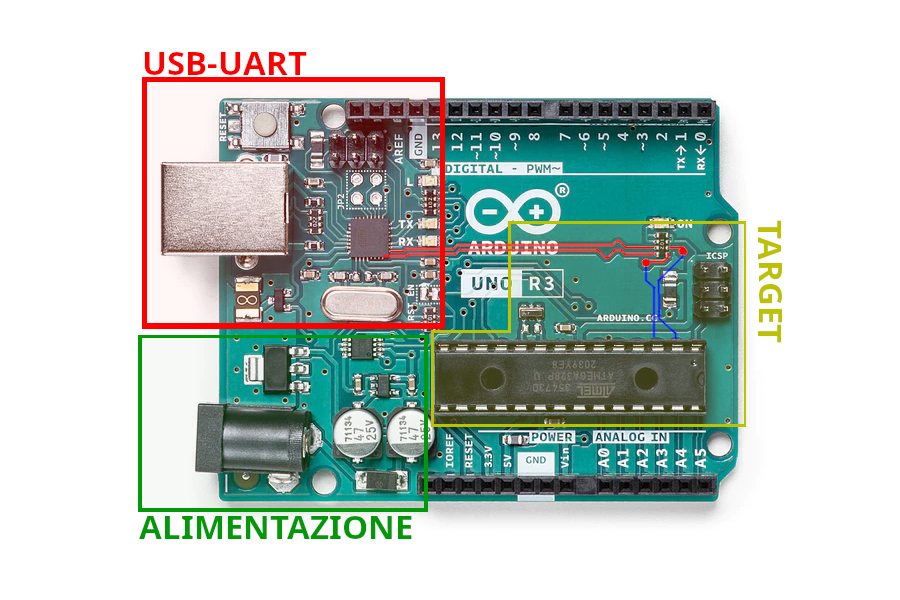
\includegraphics[width=.55\textwidth]{arduino-uno.png}
    \caption[]{Foto di una scheda Arduino Uno R3\cite{img:arduino-uno-r3}}\label{fig:arduino-uno-r3}
\end{figure}

Il controllore, presente al centro della scheda, in un involucro DIP-28\footnote{Dual in-line package, 28 pin}, è un ATMega328P-PU\cite{site:arduino-uno-doc}. La scelta di un involucro ingombrante, in controtendenza con i processi di miniaturizzazione dell'industria elettronica, è causata dal fatto che, per mantenere una dinamica ``\textit{user friendly}'', rende possibile sostituire il controllore in caso di guasto in modo semplice senza dover sostituire l'intera scheda essendo il controllore posto in uno zoccolo invece che saldato direttamente alle connessioni\cite{site:arduino-uno-doc}.

\section{La famiglia AVR}

Il controllore ATMega328P-PU presente sulla scheda di sviluppo è un membro della famiglia AVR di Atmel\cite[1]{avr:m328p}.

Come è possibile identificare dalla \cref{fig:avr-arch} l'architettura del processore della famiglia AVR è di tipo Harvard: è evidente la dicotomia tra memoria del programma (nell'immagine ``\textit{Flash Program Memory}'') e SRAM\cite{harvard-arch}. Questa suddivisione consente di ottimizzare separatamente le due diverse tecnologie di memorie intrinsecamente diverse.

È inoltre possibile osservare che la grandezza del bus dati è di 8 bit: conseguentemente è possibile dedurre che l'intera architettura si basa sull'unità fondamentale del byte.

La maggior parte delle istruzioni viene eseguita in un solo ciclo di clock\cite[sec 7.6]{avr:m328p} --- essendo un processore con pipeline a due stadi è possibile eseguire il fetch dell'istruzione successiva durante l'esecuzione corrente --- ad esclusione delle operazioni sulle memorie le quali ``stallano'' il processore per questioni di tempi di accesso/scrittura, di istruzioni che coinvolgono dati di lunghezza maggiore di 8 bit oppure istruzioni che implicano il ripristino della pipeline come le istruzioni di salto o lettura della memoria flash.

\begin{figure}[t]
    \centering
    %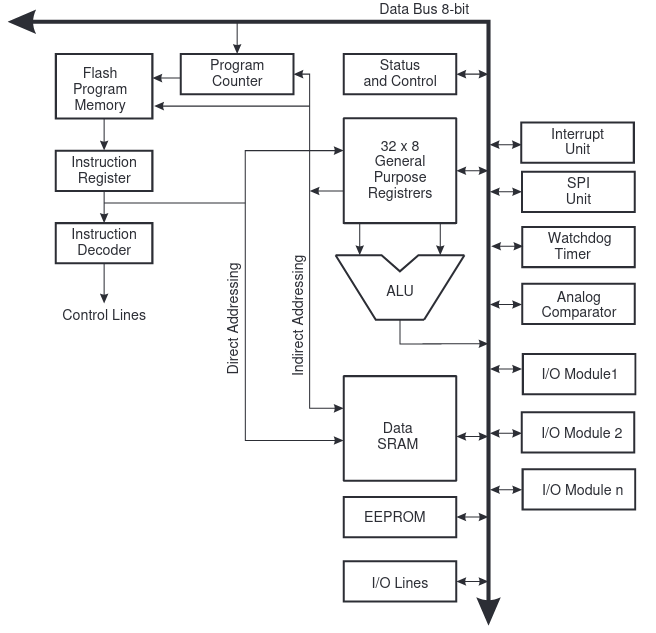
\includegraphics[width=.9\textwidth]{avr_arch.png}
    \includegraphics[page=18, width=.9\textwidth,trim={30mm 67mm 30mm 70mm},clip]{../biblio/docs/m328.pdf}
    \caption[Immagine ottenuta dal documento~\cite{avr:m328p} fig 7-1]{Schema a blocchi dell'architettura AVR\cite[fig 7-1]{avr:m328p}}\label{fig:avr-arch}
\end{figure}

\subsection{Funzionalità avanzate}\label{ss:advanced-features}

Per i micro controllori di fascia media esiste la differenziazione tra codice di bootloader e codice eseguibile.

Il codice ``privilegiato'', il bootloader, può essere eseguito se si verificano determinati eventi rilevabili dall'hardware quali condizioni di reset particolari o al verificarsi di una condizione sullo stato di un pin; oppure può essere protetto da sovrascrittura/lettura con criteri diversi dal codice dell'applicazione ed è in grado di riprogrammare la memoria dello stesso integrato mentre è in esecuzione (Read While Write)\cite[sec 27.4]{avr:m328p}. Al contrario, il codice applicativo è destinato alla sola esecuzione.

\subsection{Memorie}

All'interno di un controllore della famiglia AVR, essendo un processore ad architettura harvard, è possibile trovare due diverse tipologie di memorie dedicate --- utili all'ottimizzazione di costi e funzionamento --- e una terza tipologia dedicata all'utilità e alla riduzione dei costi dell'hardware (EEPROM).

\subsubsection{Memoria FLASH}
La memoria flash è dedicata alla conservazione del codice eseguibile.
Dato l'utilizzo generale di sola lettura, essa si presenta come una memoria a lettura veloce, organizzata ad unità elementari di 16 bit --- dimensione minima degli opcode\cite{avr:isa} --- e riprogrammabile a pagine.

Si tratta poi di una memoria complessa: per i controllori avanzati, aventi il supporto al bootloader, essa è divisa in due sezioni le quali garantiscono la possibilità di differenziare i privilegi del codice presente nelle due sezioni come descritto nella \cref{ss:advanced-features}.

Essendo inoltre una memoria ``di programma'', essa non richiede prestazioni notevoli in scrittura: questa avviene, come detto precedentemente, a pagine, ossia a blocchi di 512/1024 bit (in funzione del controllore e della dimensione della memoria) e può essere eseguita in tre diverse modalità:

\begin{itemize}
    \item ISP\footnote{In System Programming}: In questo caso il controllore è in modalità di programmazione ed esegue i comandi inoltrati da un programmatore esterno --- connesso tramite SPI\footnote{Serial Peripheral Interface} --- mentre la CPU è in stato di \textit{halt}.
    \item Self Programming: Grazie all'istruzione \texttt{spm} è possibile riprogrammare le pagine della memoria flash dall'interno del codice stesso\footnote{Nel caso in cui sia presente il supporto al bootloader, \texttt{spm} può essere eseguito solo se il program counter punta a tale regione.}.
    \item High Voltage Parallel Programming: Viene utilizzato in caso la linea di reset sia configurata con una funzione ausiliaria: consiste nell'applicare +12V sulla pin di reset forzando la modalità di programmazione parallela a discapito della configurazione del pin\cite[sec 28.6]{avr:m328p}.
\end{itemize}

\subsubsection{EEPROM}

La memoria EEPROM\footnote{Electrically Erasable and Programmable Read-Only Memory} è considerata una memoria di utilità in quanto non necessariamente essenziale alla vita del codice in esecuzione. Essa permette di salvare dati in modo non volatile nell'eventualità di una mancanza di alimentazione.

Si tratta di una memoria ``lenta'' (tempi di programmazione di 3.4ms\cite[tab 8-1]{avr:m328p}) ma in grado di essere letta e scritta con un'unità fondamentale di 8 bit\cite[sec 8.4]{avr:m328p} e garantire una vita dieci volte più duratura in termini di scritture rispetto alla memoria flash precedentemente descritta\cite[sec 8.2, sec 8.4]{avr:m328p}.

Il vantaggio che si presenta con l'integrazione di tale memoria all'interno dell'micro-controllore consiste nell'eliminazione di un ulteriore componente sul circuito stampato e una riduzione dei costi nel caso essa sia necessaria, oltre al non utilizzo di una periferica di comunicazione dedicata a tali scopi.

L'interazione con la memoria avviene tramite la scrittura e lettura dei registri \texttt{EECR} \texttt{EEDR} \texttt{EEARL/H} (EEPROM Control, Data e Address Registers)\cite[34]{avr:m328p}.

\subsubsection{SRAM}
La memoria SRAM\footnote{Static Random Access Memory} è uno dei componenti di maggiore importanza della struttura dell'integrato.

Essa consiste nella principale memoria di elaborazione, ma la sua struttura è leggermente più complessa rispetto a quanto si possa trovare su un comune calcolatore.
Infatti l'architettura AVR utilizza in modo marcato il concetto di MMIO\footnote{Memory Mapped Input and Output}.

\begin{figure}[b]
    \centering
    \includegraphics[page=28, width=.7\textwidth,trim={70mm 90mm 40mm 145mm},clip]{../biblio/docs/m328.pdf}
    \caption[Immagine ottenuta dal documento~\cite{avr:m328p}, fig. 8-3]{Settorizzazione della memoria SRAM del controllore ATMega328P\cite[fig 8-3]{avr:m328p}}\label{fig:avr-sram-alloc}
\end{figure}

Come è possibile osservare dalla \cref{fig:avr-sram-alloc}, i primi 256 byte dello spazio degli indirizzi della memoria SRAM sono in realtà dedicati all'interazione con registri di controllo delle periferiche.

Questi vengono identificati da un indirizzo nella memoria SRAM ma sono in realtà collocati nelle varie periferiche che essi controllano il cui accesso avviene sfruttando le linee di controllo per la scrittura della memoria SRAM\cite[fig 14-2]{avr:m328p}.

La scrittura di tali locazioni di memoria causa effetti collaterali in funzione della periferica alla quale è associata. Questa sezione si divide in tre blocchi: i primi 32 byte sono i registri \textit{general purpose} i quali sono interconnessi e interagiscono con l'ALU.\@ Essi vengono utilizzati per l'elaborazione e il salvataggio di dati temporanei.

A seguire sono presenti due zone di memoria: \textit{I/O} ed \textit{Extended I/O} contenenti i registri di controllo delle periferiche. A tal fine, dato che le scritture e le letture possono causare cambiamenti alla periferica (e.g.\ la scrittura di un flag di interrupt per ripristinare lo stato di una periferica) questi indirizzi vengono dichiarati mediante la keyword \texttt{volatile}\footnote{Keyword del compilatore C per impedire l'ottimizzazione delle letture e scritture ad un dato indirizzo}. La differenza tra le due sezioni consiste nella possibilità della prima di essere acceduta in un solo ciclo di clock tramite le istruzioni di \textit{I/O}\cite[sec 8.5]{avr:m328p} quali \texttt{in}, \texttt{out}, ecc\ldots

È possibile notare dalla \cref{fig:avr-sram-timings} come le istruzioni di accesso alla ram impieghino due cicli di clock: l'indicizzazione della ram da parte di alcune istruzioni è effettuata utilizzando il valore composto da una coppia di registri\footnote{r26-r27, r28-r29, r30-r31} al momento dell'esecuzione. 

Queste operazioni possono indirizzare la SRAM tramite il valore presente nei registri dedicati oltre alla possibilità di fare pre-incremento e post-incremento del valore contenuto in tali indirizzi.

\begin{figure}[b]
    \centering
    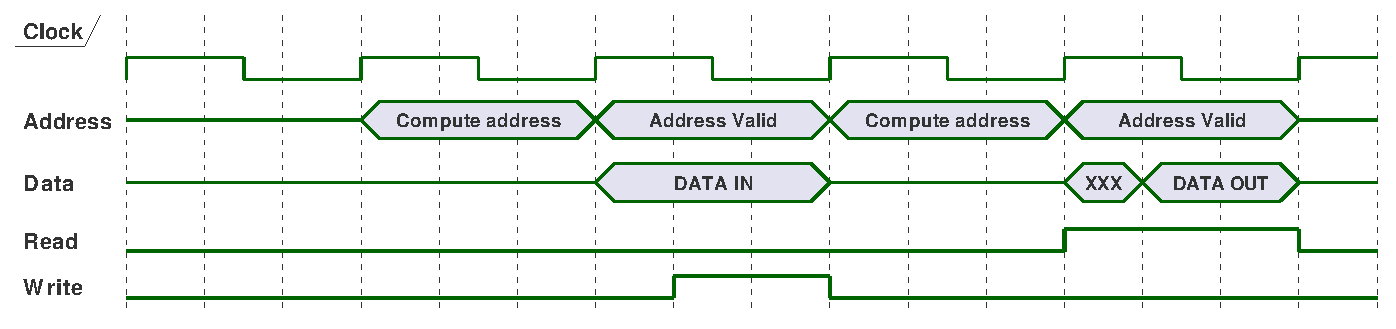
\includegraphics[width=.9\textwidth]{avr-sram-timings.pdf}
    \caption[Immagine rielaborata a partire dalla fig. 8-4 del documento~\cite{avr:m328p}]{Sequenze di accesso in lettura e scrittura della memoria SRAM\cite[fig 8-4]{avr:m328p}}\label{fig:avr-sram-timings}
\end{figure}

In particolare, un uso comune delle istruzioni di accesso alla memoria viene mostrato dal \cref{lst:store-example}, riga 6.

\noindent\begin{minipage}{\textwidth}
    \begin{lstlisting}[language=AVR, caption={Esempio di utilizzo dell'istruzione \texttt{st}}, label=lst:store-example]
        ldi r24, 0xFF ;Salva la costante 0xFF nel registro r24
        eor r0, r0 ;Salva la costante 0x00 nel registro r0
        eor r26, r26 ;Azzera il contenuto di r26 (XL)
        eor r27, r27 ;Azzera il contenuto di r27 (XH)
    loop:
        st r24, X+ ;SRAM[r27:r26] = r24
        dec r24 ;r24--
        cpse r24, r0 ;if(r24 == 0) goto hold
        rjmp loop ;else goto loop
    hold:
        rjmp hold ;goto hold

    \end{lstlisting}
\end{minipage}

Il codice presentato dal \cref{lst:store-example}, mostra nelle linee 1-4 l'azzeramento dei registri r0, r26 e r27 (dove gli ultimi due elencati vengono definiti nel codice dal meta-registro X) e in seguito definisce un ciclo dove viene salvato il contenuto di r24 all'indirizzo puntato dal registro X con successivo incremento; segue l'istruzione \texttt{cpse}\footnote{Compare and Skip if Equal} la quale compara rispetto alla costante 0 il valore di r24 una volta decrementato. Nel caso in cui la comparazione risulti veritiera, viene incrementato il program counter di due \textit{word}, terminando quindi l'esecuzione nel ciclo di \textit{hold}.

\section{La scheda}
Come menzionato ad inizio capitolo, la scheda utilizzata nello sviluppo del sistema è \textit{Arduino Uno R3}.

È possibile notare come nello schema elettronico della scheda (\ref{app:r3-schematic}) siano presenti due distinti componenti principali e tre sezioni funzionali diverse.

\subsection{Circuito di alimentazione}

Il circuito di gestione dell'alimentazione della scheda si occupa di fornire la tensione adeguata al funzionamento dei due micro-controllori e di utilizzare la sorgente più adatta.

Le due sorgenti di alimentazione della scheda si identificano nel componente \texttt{X1} e nella porta USB \texttt{X2}. Data la presenza di due possibili sorgenti delle quali la prima presenta un input non regolato --- in quanto il componente \texttt{X1} consiste in una presa di alimentazione cilindrica collegata al pin 3 di un regolatore di tensione con intervallo di funzionamento dell'ingresso da \SI{7}{\volt} a \SI{20}{\volt}\cite{onsemi:ncp111750} --- si rende necessario un circuito di selezione mostrato dalla \cref{fig:r3-schematic-pwr-sel-detail}.

\begin{figure}[t]
    \centering
    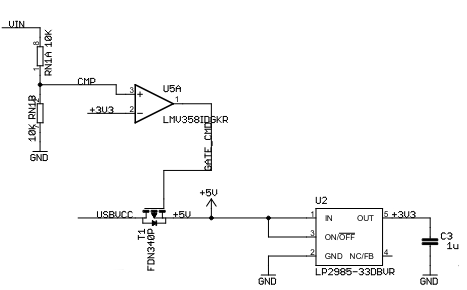
\includegraphics[width=.8\textwidth]{r3-schematic-pwr-sel.png}
    \caption[Dettaglio dello schema elettronico posto in appendice, documento~\ref{app:r3-schematic}]{Dettaglio dello schema elettronico della scheda Arduino Uno R3, documento~\ref{app:r3-schematic}~\cite{site:r3-schematic}}\label{fig:r3-schematic-pwr-sel-detail}
\end{figure}

Per analizzare il circuito presentato dalla \cref{fig:r3-schematic-pwr-sel-detail} è necessario ipotizzare diversi scenari iniziali.

Ipotizzando il caso in cui la scheda venga collegata ad una sorgente di alimentazione esterna maggiore di \SI{7}{\volt} tramite il connettore \texttt{X1}, si ha che il collegamento \texttt{USBVCC} avrà tensione pari a \SI{0}{\volt}.
L'ingresso, inoltre, alimenterà il componente \texttt{U1} (non mostrato in figura) che regolerà la tensione e alimenterà la linea \texttt{+5V}, la quale alimenterà il componente \texttt{U2} che, a sua volta, alimenterà la linea \texttt{+3V3}.
Il comparatore (\texttt{U5A}) avrà uscita a \SI{5}{\volt} se \texttt{VIN} --- collegato direttamente alla sorgente esterna tramite un diodo (\texttt{D1}) --- è superiore a \SI{6.6}{\volt}: l'uscita del comparatore pilota il gate del mosfet a canale P \texttt{T1} non avendo però alcun effetto in quanto, come detto precedentemente, \texttt{USBVCC} è posto a \SI{0}{\volt}.

Ipotizzando ora il caso in cui la scheda è solamente collegata a un computer tramite la porta USB si avrà che la connessione \texttt{VIN} avrà potenziale \SI{0}{\volt}.

\texttt{USBVCC} avrà potenziale \SI{5}{\volt} da specifica USB\cite{usb2.0specs}.\@ In una fase iniziale la linea \texttt{+5V} avrà quindi potenziale pari a \SI{4.3}{\volt} considerando la caduta di tensione del diodo presente all'interno del componente \texttt{T1}; tensione sufficiente ad alimentare il comparatore \texttt{U5A} e il regolatore di tensione \texttt{U2}.
Essendo \texttt{VIN} posta a \SI{0}{\volt}, l'uscita del comparatore sarà anch'essa posta a tale tensione --- essendo il componente LMV358 un amplificatore operazionale \textit{rail-to-rail}\cite{ti:lmv358} --- stabilendo una differenza di potenziale tra il gate e il source di \SI{5}{\volt} abbattendo così la resistenza equivalente del mosfet \texttt{T1} e portando la linea di alimentazione a \SI{5}{\volt} effettivi\cite{onsemi:fdn340p}.

Ipotizzando infine che, data la condizione stabile precedentemente descritta, l'utente colleghi la scheda a una seconda sorgente (tramite \texttt{X1}) contemporaneamente all'alimentazione USB, se la tensione VIN è superiore a \SI{6.6}{\volt}, l'uscita del comparatore \texttt{U5A} incrementerà a \SI{5}{\volt}, causando così una differenza di potenziale gate-source per il componente \texttt{T1} di \SI{0}{\volt} e di conseguenza la ``disconnessione'' del carico da \texttt{USBVCC}.

\subsection{Comunicazione con l'host}

Il caricamento e la comunicazione tra \textit{target} e \textit{host} avvengono tramite una linea seriale UART.\@ Ne consegue il problema di adattare un'interfaccia seriale TTL, non presente su un computer \textit{consumer grade}, a una presente sulle comuni piattaforme di elaborazione.

Questa funzionalità viene svolta dal componente \texttt{U3} dello schema allegato (\ref{app:r3-schematic}). Esso è un microcontrollore della famiglia AVR con il supporto USB.\@

In particolare si tratta di un \texttt{ATMega16U2} con caricato un firmware implementante la classe CDC del protocollo USB, rendendo il dispositivo una periferica RS232 virtuale.
Il firmware si occupa di ricevere i dati dall'\textit{host} e di replicarli sulla linea seriale (pin 8 e 9) e vice versa.\cite[firmwares/atmegaxxu2/arduino-usbserial/]{git:arduinocore}.

\begin{figure}[t]
    \centering
    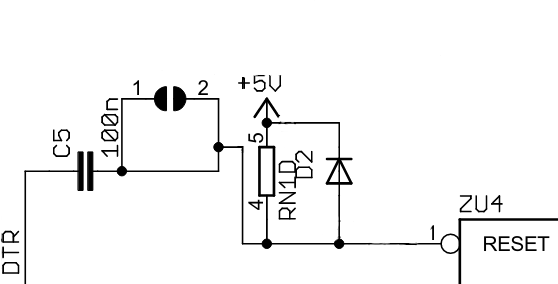
\includegraphics[width=.8\textwidth]{r3-rst-cap.png}
    \caption[Dettaglio dello schema elettronico posto in appendice, documento~\ref{app:r3-schematic}]{Dettaglio della connessione alla linea di reset dell'ATMega16U2, documento \ref{app:r3-schematic}~\cite{site:r3-schematic}}\label{fig:r3-schematic-rst-detail}.
\end{figure}


Oltre alle connessioni relative alla comunicazione seriale tra \textit{target} e l'ATMega16U2 (\texttt{M8TXD} e \texttt{M8RXD}) è presente una terza connessione che pilota la linea di reset del primo. Il pin 13 dell'ATMega16U2 è connesso, tramite \texttt{C5} alla linea di reset del \textit{target}.

Secondo la specifica RS-232, oltre alle due linee seriali, sono presenti anche delle line di ``\textit{flow control}'', tra le quali possiamo notare la linea attiva a livello logico 0 nominata \texttt{``DTR''}.

Questa linea è asserita dalla maggior parte dei driver seriali (e seriali virtuali) al momento della connessione al dispositivo o del collegamento. Così facendo, grazie a \texttt{C5} è possibile avere un impulso sulla linea di reset prima che il circuito ritorni all'equilibrio: Inizialmente il condensatore \texttt{C5} si trova in equilibrio con la linea DTR posta a \SI{5}{\volt} e la linea di RESET posta a \SI{5}{\volt} per mezzo della resistenza di pull'up. Al momento dell'asserzione la linea DTR viene posta a \SI{0}{\volt} e conseguentemente il condensatore \texttt{C5} si carica causando un calo nella linea di reset fino a \SI{0}{\volt}, la quale poi evolverà secondo il modo del sistema dato dal prodotto tra la resistenza e la capacità di \texttt{RN1D} e \texttt{C5} equivalente a quanto riportato nell'~\cref{eq:rcstrrst}.

\begin{equation}\label{eq:rcstrrst}
    \tau_{reset} = \frac{1}{\text{RN1D} \cdot \text{C5}} = \SI{1}{\milli\second}
\end{equation}

Al momento della disconnessione il condensatore causerà un picco positivo nella linea di reset fino a circa \SI{10}{\volt} che verrà però soppresso dalla presenza di \texttt{D2} limitandolo a \SI{5.7}{\volt} senza eccedere i limiti fisici del pin con il quale è collegato.

\subsection{Programmazione}

La programmazione dell'integrato \textit{target} non avviene secondo i metodi tradizionali ma attraverso un bootloader pre-caricato\cite[bootloaders/atmega/ATmegaBOOT\_168.c]{git:arduinocore}. 
Una volta forzato il reset tramite l'asserzione della linea \texttt{DTR} il bootloader viene attivato e, in caso di ricezione di comandi di programmazione, esso inizia la programmazione tramite l'istruzione \texttt{spm}.

